\setchapterpreamble[u]{\margintoc}
\chapter{2-Dimensional Potential}

We will worked with the harmonic oscilator again, but this time in 2 spatial dimensions.

\section{Classical Mechanics}

As we did in chapter 1 we want to understand first the behaviour of the classical mechanics for the problem.

The potential V(x,y) is:

\begin{equation}
  V(x,y) = \frac{1}{2} k (x^2+y^2) = \frac{1}{2} k \rho^2
\end{equation}

The math becomes easier if we used polar coordinates as we did in Chapter 1. In this coordinates the energy is:

\begin{equation}
  E = \frac{1}{2} m \left(\frac{\partial \rho}{\partial t}\right)^2 + \frac{L^2}{2m\rho^2} + \frac{1}{2}k \rho^2
\end{equation}

We are going to solve for the change among time in $\rho$ to solve the problem.

\begin{equation}
  \begin{array}{c}
    \frac{\partial \rho}{\partial t} = \sqrt{\frac{2}{m}\left(E-\frac{L^2}{2 m \rho^2}-\frac{1}{2}k\rho^2\right)}
    \\

    \\
    \frac{\partial \rho}{\partial t} = \sqrt{\frac{k}{m\rho^2}\left(\frac{2E}{k}\rho^2-\frac{L^2}{m k}-\rho^4\right)}
  \end{array}
\end{equation}

Using equation 7.2 we can turn the previous equation into:

\begin{equation}
  \begin{array}{c}
    \frac{\rho}{\omega}\frac{\partial \rho}{\partial t} = \sqrt{\frac{2E}{m^2\omega^2}\rho^2 - \frac{L^2}{m \omega^2}-\rho^4}
  \end{array}
\end{equation}

We are going to change the variable $\rho$ to $u$, where $u=\rho^2$. Solving for u the equation turns into:

\begin{equation}
  \begin{array}{c}
    \frac{1}{2\omega}\frac{\partial u}{\partial t} = \sqrt{- \frac{L^2}{m \omega^2}+ \frac{2E}{m^2\omega^2}u -u^2}
    \\

    \\
    \frac{1}{2\omega}\frac{\partial u}{\partial t} = \sqrt{\left(\frac{E^2}{m^2\omega^4} - \frac{L^2}{m^2\omega^2}\right)-\left(u-\frac{E}{m\omega}\right)^2}
    \\

    \\
    \frac{1}{2\omega}\frac{\partial u}{\partial t} = \sqrt{\frac{1}{m^2\omega^4}\left(E^2-L^2\omega^2\right)-\left(u-\frac{E}{m\omega^2}\right)^2}
  \end{array}
\end{equation}

The function inside of the square root needs to be positive, which make us say than the left parenthesis is greater than the right one that is always greater than 0, i. e. :

\begin{equation}
  \begin{array}{c}
    (E^2-L\omega^2) \geq 0
    \\

    \\
    E \geq L\omega
  \end{array}
\end{equation}

We know now that there is a minimum energy, which energy is $E=L\omega$. Whenthe energy is at it's minimum is easy to get u(t):

\begin{equation}
  \begin{array}{c}
    u(t) = \frac{E}{m\omega^2} = constant
    \\

    \\
    \frac{\partial u}{\partial t} = 0
  \end{array}
\end{equation}

To analize the rest of the solution for the Energy we are going to change some of the variables by some unitless variables.

\begin{equation}
  \label{8.8}
  \begin{array}{c}
    E = \alpha L \omega
    \\

    \\
    u = \beta \frac{E}{m\omega^2}
    \\

    \\
    \omega t = \tau
  \end{array}
\end{equation}

From the previous analysis of the minimum energy we can say that $\alpha \geq 1$. Now that we have our new parameters well define we can rewrite the expression we have been working with.

\begin{equation}
  \begin{array}{c}
    \frac{\alpha L}{m\omega}\frac{1}{2} \frac{\partial \beta}{\partial \tau} = \sqrt{\frac{L^2\omega^2}{m^2\omega^4}[\alpha^2-1]-\frac{\alpha^2 L^2}{m^2\omega^2}[\beta-1]^2}
    \\

    \\
    \frac{1}{2} \frac{\partial \beta}{\partial \tau} = \sqrt{\left(1-\frac{1}{\alpha^2}\right)-(\beta-1)^2}
  \end{array}
\end{equation}

Knowing that alpha is a fixed constant we can solve this equation. But first i will make the math simpler by saying $A = \left(1-\frac{1}{\alpha^2}\right)$

\begin{equation}
  \begin{array}{c}
    \frac{\partial \beta}{2\sqrt{A-(\beta-1)^2}} = \partial\tau
  \end{array}
\end{equation}

To solve the integral we have to define the limits; for $\tau$ as it is a measure of time is going to start at $\tau=0$ and end in a general $\tau$, but for $\beta$ it can start at any arbitrary $\beta \geq 0$, so we will say that $\beta$ goes from $\beta_0$ to a general $\beta$.

\begin{equation}
  \begin{array}{c}
    \int_{\beta_0}^{\beta}\frac{\partial \beta'}{2\sqrt{A-(\beta-1)^2}} = \int_{0}^{\tau}\partial\tau'
  \end{array}
\end{equation}

This integral can be solved directly if we change the variable beta and the constant A by $f = \beta-1$ and $A = B^2$.

\begin{equation}
  \begin{array}{c}
    \int_{f_0+1}^{f+1}\frac{\partial f'}{2\sqrt{A-f'^2}} = \int_{0}^{\tau}\partial\tau'
    \\

    \\
    \int_{f_0+1}^{f+1}\frac{\partial f'}{2\sqrt{A(1-\frac{f'^2}{A}}} = \int_{0}^{\tau}\partial\tau'
    \\

    \\
    \int_{f_0+1}^{f+1}\frac{B \partial f'}{2\sqrt{(1-\frac{f'^2}{B^2}}} = \int_{0}^{\tau}\partial\tau'
  \end{array}
\end{equation}

This last integral can be solved directly and it will give us the result for $f(\tau)$ and then we can recover the solution for $\beta(\tau)$.

\begin{equation}
  \begin{array}{c}
    \arcsin(\frac{f+1}{B}) - \arcsin(\frac{f_0}{B}) =2\tau
    \\

    \\
    \beta(\tau) = B \sin\left(2\tau + \arcsin\left(\frac{\beta_0}{B}\right) \right)
    \\

    \\
    \beta(\tau) = \sqrt{1-\frac{1}{\alpha^2}} \sin\left(2\tau + \arcsin\left(\frac{\beta_0}{\sqrt{1-\frac{1}{\alpha^2}}}\right) \right)
  \end{array}
\end{equation}

This is our final solution for $\beta$, from this solution we can get $\rho(t)$ by undoing the changes of variables in \ref{8.8}.

\begin{marginfigure}[-2cm]
  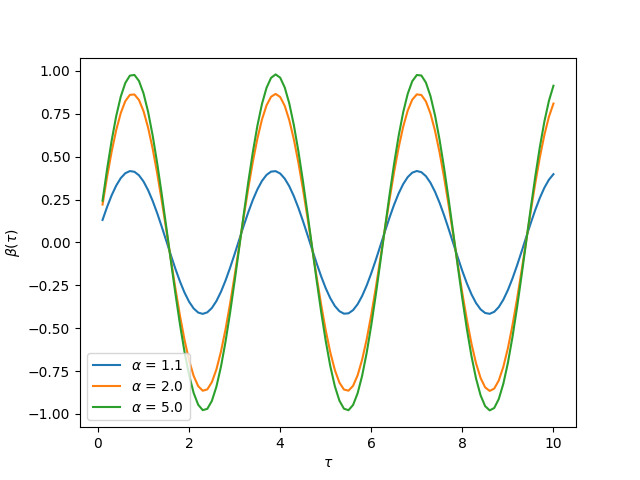
\includegraphics{images8/beta_tau.png}
  \caption{$\beta(\tau)$ function for different values of alpha}
  \labfig{beta_tau}
\end{marginfigure}

We can not forget about the other variable, the angle $\phi$. To solve for phi we will used the definition of the angular momentum.

\begin{equation}
  \begin{array}{c}
    L = m \rho^2 \frac{\partial \phi}{\partial t}
    \\

    \\
    \frac{\partial \phi}{\partial t} = \frac{L}{m \rho^2}
    \\

    \\
    \frac{\partial \phi}{\partial \tau} = \frac{1}{\alpha \beta(\tau)}
  \end{array}
\end{equation}

We want to find the solution for $\beta (\phi)$.

\begin{equation}
  \begin{array}{c}
    \frac{\partial\beta}{\partial\phi} = \frac{\frac{\partial\beta}{\partial\tau}}{\frac{\partial\phi}{\partial\tau}} = 2\alpha\beta\sqrt{\left(1-\frac{1}{\alpha^2}-(\beta-1)^2\right)}
  \end{array}
\end{equation}

Solving this equation we end up with:

\begin{equation}
  \begin{array}{c}
    \beta(\phi) = 1+\sqrt{\left(1-\frac{1}{\alpha^2}\right)} \sin\left(\frac{1}{\alpha}\tan(\phi)\right)
  \end{array}
\end{equation}

We can turn beta into rho by undoing the changes of variables in \ref{8.8}.

\begin{equation}
    \rho(\phi) = \sqrt{\beta(\phi)\frac{E}{m\omega^2}} = \sqrt{\beta(\phi)\alpha \r}
\end{equation}

In the figure below we can see the orbital movement of the particle for different values of $\alpha$.

\begin{figure}
  \centering
  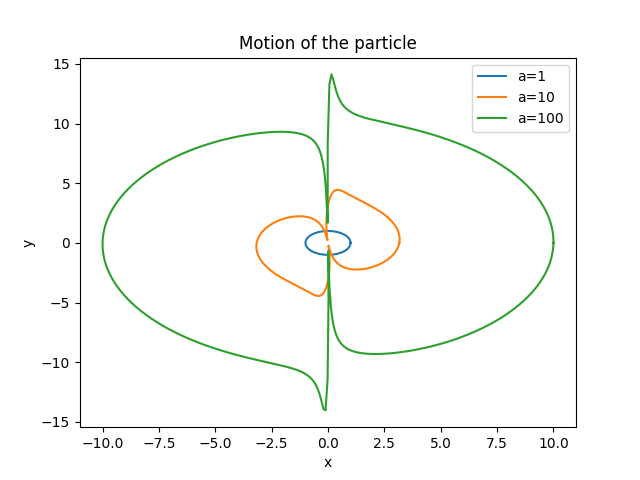
\includegraphics{images8/beta_theta.png}
  \caption{Orbital movement of the particle for different values of $\alpha$}
\end{figure}

\section{Quantum Mechanics}

We are going to solve the problem using the Schrödinger wave equation.

\begin{equation}
  \begin{array}{c}
    -\frac{\hbar^2}{2m} \left[\frac{\partial^2\phi}{\partial x^2} + \frac{\partial^2\phi}{\partial y^2}\right] + \frac{1}{2} m \omega^2 (x^2+y^2)\phi = E \phi
  \end{array}
\end{equation}

In this case we are not going to solve the problem in polar coordinates, we are going to solve it in cartesian coordinates. First, we have to set the equation to natural units.

\begin{equation}
  \begin{array}{c}
    x = b u
    \\

    \\
    y = b v
    \\

    \\
    b^2 = \frac{\hbar}{m\omega}
    \\

    \\
    \phi(x=bu,y=bv) = \psi(u,v)
  \end{array}
\end{equation}

Our wave equation now is:

\begin{equation}
  \begin{array}{c}
    -\frac{1}{2}\hbar\omega \left[\frac{\partial^2\psi}{\partial u^2} + \frac{\partial^2\psi}{\partial v^2}\right] + \frac{1}{2} \hbar \omega (u^2+v^2)\psi = E \psi
  \end{array}
\end{equation}

As we did in the classical aproach we are going to change the energy by $E=\alpha\hbar\omega$. The wave equation now looks like:

\begin{equation}
  \begin{array}{c}
    \left[-\frac{1}{2}\left(\frac{\partial^2}{\partial u^2}+\frac{\partial^2}{\partial v^2}\right)+\frac{1}{2}(u^2+v^2)\right]\psi = \alpha \psi
  \end{array}
\end{equation}

As we did in one dimension we can use some operators to solve this equation. We are going to define this as:

\begin{equation}
  \begin{array}{c}
    a_u = \frac{1}{\sqrt{2}}\left[\frac{\partial}{\partial u}+u\right]
    \\

    \\
    a_v = \frac{1}{\sqrt{2}}\left[\frac{\partial}{\partial v}+v\right]
    \\

    \\
    a_u^{\dagger} = \frac{1}{\sqrt{2}}\left[-\frac{\partial}{\partial u}+u\right]
    \\

    \\
    a_v^{\dagger} = \frac{1}{\sqrt{2}}\left[-\frac{\partial}{\partial v}+v\right]
  \end{array}
\end{equation}

It can be proved that $a a^{\dagger}$ is an hermitian operator of $\chi$ for any of the variables; u,v.

We have also similar relations to the ones we had in one dimension.

\begin{equation}
  \begin{array}{c}
    \left[a_u,a_u^{\dagger}\right] = 1
    \\

    \\
    \left[a_v,a_v^{\dagger}\right] = 1
    \\

    \\
    \left[a_u,a_v\right] = 0
    \\

    \\
    \left[a_u^{\dagger},a_v^{\dagger}\right] = 0
    \\

    \\
    N_u = a_u^{\dagger}a_u
    \\

    \\
    N_v = a_v^{\dagger}a_v
    \\

    \\
    \left[N_u,a_u^{\dagger}\right] = a_u^{\dagger}
    \\

    \\
    \left[N_u,a_u\right] = -a_u
    \\

    \\
    \left[N_v,a_v^{\dagger}\right] = a_v^{\dagger}
    \\

    \\
    \left[N_v,a_v\right] = -a_v
  \end{array}
\end{equation}

The commutator of any two cross operators is 0. With this we end up with the following equation:

\begin{equation}
  \begin{array}{c}
    \left[N_u+N_v\right] \psi = (\alpha-1) \psi
  \end{array}
\end{equation}

Which means that $\alpha \geq 1$, as it was in classical mechanics. We can use the operators $a_u^{\dagger}$ or $a_v^{\dagger}$ to get the next level of energy for the equation.

\begin{equation}
  \begin{array}{c}
      \left[N_u+N_v+1\right] (a^{\dagger}\psi) = \left[a^{\dagger}N_u + a^{\dagger} + a^{\dagger}N_v \right]
      \\

      \\
      \left[N_u+N_v+1\right] (a^{\dagger}\psi) = a^{\dagger}[N_u+N_v+1]\psi
      \\

      \\
      \left[N_u+N_v+1\right] (a^{\dagger}\psi) = (\alpha+1-1)a^{\dagger}\psi
  \end{array}
\end{equation}

The operator $a^{\dagger}$ could be either of the two posible operators, and the result is the same. We can say that the operator $a^{\dagger}$ is giving us the next level of energy for the equation, $\alpha$ increases by one.

There is an $\alpha = 1$, which is the minimum energy for the system, which means that there is a lower energy state $\psi_0$ where:

\begin{equation}
  \begin{array}{c}
    \left[N_u+N_v\right] \psi_0(u,v) = 0
  \end{array}
\end{equation}

So:

\begin{equation}
  \begin{array}{c}
    a_u \psi_0(u,v) = 0
    a_v \psi_0(u,v) = 0
  \end{array}
\end{equation}

There must be a function $\psi_0(u,v)$ that satisfies this two equations. Let's try to solve it.

\begin{equation}
  \begin{array}{c}
    \left(\frac{\partial}{\partial u} + u\right)\psi_0(u,v) = 0
    \\

    \\
    \left(\frac{\partial}{\partial v} + v\right)\psi_0(u,v) = 0
  \end{array}
\end{equation}

The solution for this equation is:

\begin{equation}
  \begin{array}{c}
    \ln\psi_0(u,v) + \frac{1}{2}u^2 = f(v)
    \\

    \\
    \ln\psi_0(u,v) + \frac{1}{2}v^2 = f(u)
    \\

    \\
    \psi_0(u,v) = A e^{-\frac{1}{2}(u^2+v^2)}
  \end{array}
\end{equation}

Where A is the normalization factor than can be calculated by:

\begin{equation}
  \begin{array}{c}
    \int_{-\infty}^{\infty}\int_{-\infty}^{\infty} \psi_0^2(u,v) du dv = 1
    \\

    \\
    \int_{-\infty}^{\infty}\int_{-\infty}^{\infty} A^2 e^{-u^2-v^2} du dv = 1
    \\

    \\
    A^2 \int_{-\infty}^{\infty} e^{-u^2} du \int_{-\infty}^{\infty} e^{-v^2} dv = 1
    \\

    \\
    A^2 \left(\sqrt{\pi}\right)^2 = 1
    \\

    \\
    A = \frac{1}{\sqrt{\pi}}
  \end{array}
\end{equation}

This is the solution for the ground state of the system. We can now use the operator $a^{\dagger}$ to get the next level of energy even for u or for v, both states will have the same energy but different functions, i.e. $\alpha=2$ have two states $\psi_{1,0}$ and $\psi_{0,1}$.

\begin{equation}
  \begin{array}{c}
    \psi_0 = \frac{1}{\sqrt{\pi}} e^{-\frac{1}{2}(u^2+v^2)}
    \\

    \\
    A_{1,0} = a_u^{\dagger} \psi_0 = \frac{1}{\sqrt{2}}\left[-\frac{\partial}{\partial u}+u\right]\psi_0 = \frac{2}{\pi} u e^{-\frac{u^2+v^2}{2}}
    \\

    \\
    A_{0,1} = a_v^{\dagger} \psi_0 = \frac{1}{\sqrt{2}}\left[-\frac{\partial}{\partial v}+v\right]\psi_0 = \frac{2}{\pi} v e^{-\frac{u^2+v^2}{2}}
  \end{array}
\end{equation}

To determine the normalization coeficient we have to use the same procedure as before.

\begin{equation}
  \begin{array}{c}
    A^2_{1,0} = \int_{-\infty}^{\infty}\int_{-\infty}^{\infty} \psi_{1,0}^2(u,v) du dv = \frac{2}{\pi^2} \int_{-\infty}^{\infty}\int_{-\infty}^{\infty} u^2 e^{-\frac{u^2+v^2}{2}} du dv
  \end{array}
\end{equation}

To solve this integral we are going to use polar coordinates.

\begin{equation}
  \begin{array}{c}
    A^2_{1,0} = \frac{2}{\pi^2} \int_{0}^{\infty} rdr \int_{0}^{2\pi} r^2 \sin^2(\theta) e^{-r^2} d\theta =
    \\

    \\
    = \frac{1}{\pi} \int_{0}^{\infty} r^3 e^{-r^2} dr \int_{0}^{2\pi} 2\sin^2(\theta) d\theta = \frac{1}{\pi} \frac{1}{2} 2\pi = 1
  \end{array}
\end{equation}

Which means that $A^2 = 1$, so $A = e^{i\phi}$, but we are only interested in the real part of the function, so $A = 1$. We can do the same for $\psi_{0,1}$.

\marginnote{This variables are called Hidden Variables in quantum mechanics. They are not observable, but they have become important for new physics, for example in the field of quantum computation.}

We can continue this process to get the next levels of energy. The final results fo the next level are:

\begin{equation}
  \begin{array}{c}
    \psi_{2,0} = \frac{1-2u^2}{2\sqrt{\pi}}e^{-\frac{u^2+v^2}{2}}
    \\

    \\
    \psi_{0,2} = \frac{1-2v^2}{2\sqrt{\pi}}e^{-\frac{u^2+v^2}{2}}
    \\

    \\
    \psi_{1,1} = \frac{uv}{\sqrt{2\pi}}e^{-\frac{u^2+v^2}{2}}
  \end{array}
\end{equation}

The solutions can be visualized in the following figures.

\begin{figure}
  \centering
  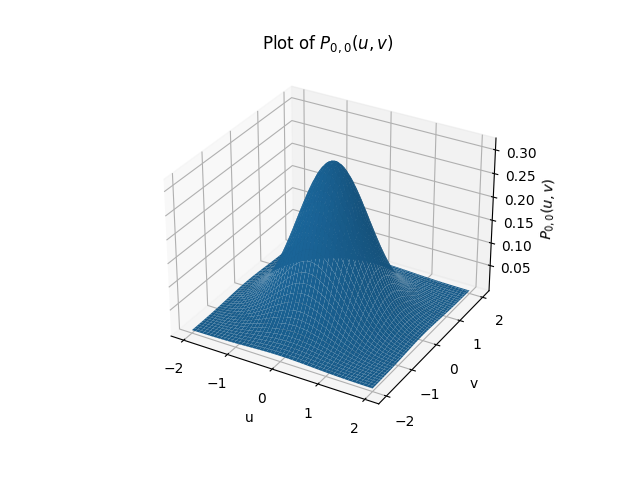
\includegraphics{images8/P_0,0.png}
  \caption{Probability distribution for the state $\psi_{0,0}(u,v)$}
\end{figure}

\begin{figure}
  \centering
  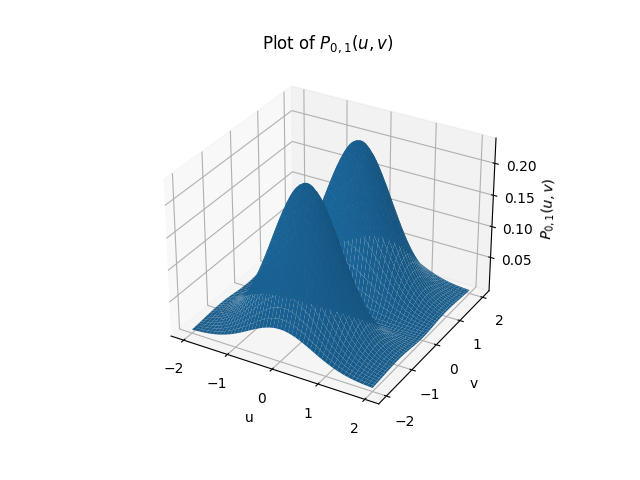
\includegraphics{images8/P_0,1.png}
  \caption{Probability distribution for the state $\psi_{0,1}(u,v)$}
\end{figure}

\begin{figure}
  \centering
  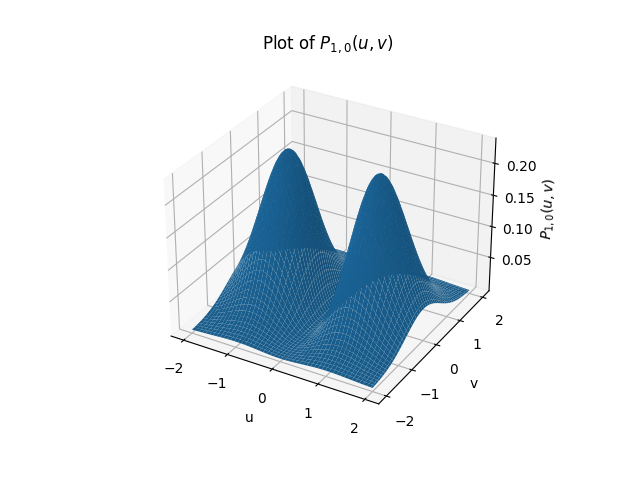
\includegraphics{images8/P_1,0.png}
  \caption{Probability distribution for the state $\psi_{1,0}(u,v)$}
\end{figure}

\begin{figure}
  \centering
  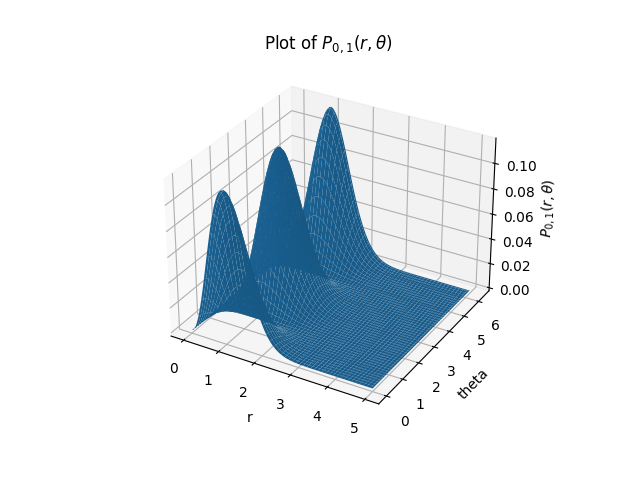
\includegraphics{images8/P_0,1(r).png}
  \caption{Probability distribution for the state $\psi_{0,1}(r,\theta)$}
\end{figure}

\begin{figure}
  \centering
  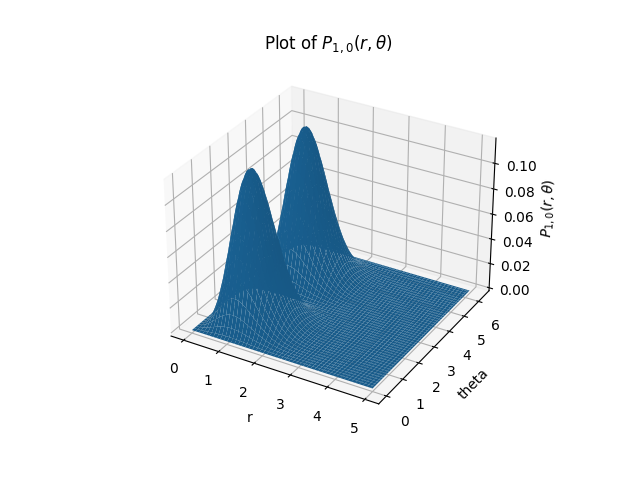
\includegraphics{images8/P_1,0(r).png}
  \caption{Probability distribution for the state $\psi_{1,0}(r,\theta)$}
\end{figure}

\section{Mixed Quantum states}

Given $\alpha = 2$ and the density Probability of a mixed state $\psi$, we can say that:

\begin{equation}
  \psi = C_{1,0} \psi_{1,0} + C_{0,1} \psi_{0,1}
\end{equation}

Where $C_{1,0}$ and $C_{0,1}$ are real numbers, (to keep it simpler). If the probability density is normalized we found:

\begin{equation}
  \begin{array}{c}
    \int_{-\infty}^{\infty} \int_{-\infty}^{\infty} \psi^{\star}(u,v)\psi(u,v) du dv = 1
    \\

    \\
    \int_{-\infty}^{\infty} \int_{-\infty}^{\infty} \left(C_{1,0} \psi_{1,0} + C_{0,1} \psi_{0,1}\right)^{\star} \left(C_{1,0} \psi{1,0} + C_{0,1} \psi{0,1}\right) du dv = 1
    \\

    \\
    \int_{-\infty}^{\infty} \int_{-\infty}^{\infty} \left(C_{1,0}^2 \psi^*_{1,0} \psi{1,0} + C_{0,1}^2 \psi^*_{0,1} \psi{0,1}\right) du dv = 1
    \\

    \\
    C_{1,0}^2 + C_{0,1}^2 = 1
  \end{array}
\end{equation}

This means that the sum of the square of the coefficients is going to be 1.

We can transform the probability into any system, we are going to choose the probability in terms of $r$ and $\theta$

\begin{equation}
  \begin{array}{c}
    P(r,\theta) = \psi^{\star}(r,\theta)\psi(r,\theta) = \left(C_{1,0} \psi^*_{1,0} + C_{0,1} \psi^*_{0,1}\right)^{\star} \left(C_{1,0} \psi{1,0} + C_{0,1} \psi{0,1}\right)
    \\

    \\
    P(r,\theta) = \frac{2}{\pi} \left(C_{1,0}^2\sin^2\theta + 2C_{1,0}C_{0,1} \sin\theta \cos\theta + C_{0,1}\cos^2\theta \right)
    \\

    \\
    P(r,\theta) = \frac{2}{\pi} \left(\frac{1}{2}+\frac{C_{0,1}^2-C_{1,0}^2}{2}\cos 2\theta + C_{1,0}C_{0,1} \sin 2\theta \right)
\end{array}
\end{equation}

This means than knowing the probability depending on the angle $\theta$ we can get the coefficients $C_{1,0}$ and $C_{0,1}$, i.e. how the state is distributed in terms of the pure quantum states.

\section{The angular momentum}

As we did in the classical mechanics we are going to solve the problem in polar coordinates.

We need to transform the variables and derivatives into a polar system.

\begin{equation}
  \begin{array}{cc}
    u = r \cos\theta & v = r \sin\theta
    \\

    \\
    du = (dr) \cos\theta - r \sin\theta d\theta & dv = (dr) \sin\theta + r \cos\theta d\theta
  \end{array}
\end{equation}

We will rename $\psi(u,v)$ to $\chi(r,\theta)$ and we want to know how the derivatives behave for $\chi$.

\begin{equation}
  \begin{array}{c}
    \frac{\partial}{\partial u} \chi= \left[\left(\frac{\partial}{\partial\theta}\right)_{r} \left(\frac{\partial \theta}{\partial u}\right)_v +\left(\frac{\partial}{\partial r}\right)_\theta \left(\frac{\partial r}{\partial u}\right)_v \right] \chi =
    \\

    \\
    = \left(\frac{-\sin\theta}{r}\frac{\partial}{\partial \theta} + \cos\theta\frac{\partial}{\partial r} \right) \chi
    \\

    \\
    \frac{\partial}{\partial v} \chi= \left[\left(\frac{\partial}{\partial\theta}\right)_{r} \left(\frac{\partial \theta}{\partial v}\right)_u +\left(\frac{\partial}{\partial r}\right)_\theta \left(\frac{\partial r}{\partial v}\right)_u \right] \chi =
    \\

    \\
    = \left(\frac{\cos\theta}{r}\frac{\partial}{\partial \theta} + \sin\theta\frac{\partial}{\partial r} \right) \chi
  \end{array}
\end{equation}

We need to the second derivative.

\begin{equation}
  \begin{array}{c}
    \frac{\partial^2}{\partial u^2} \chi = \left(\frac{-\sin\theta}{r}\frac{\partial}{\partial \theta} + \cos\theta\frac{\partial}{\partial r} \right) \left(\frac{-\sin\theta}{r}\frac{\partial}{\partial \theta} + \cos\theta\frac{\partial}{\partial r} \right) \chi =
    \\

    \\
    = \left(\frac{\sin^2\theta}{r^2}\frac{\partial^2}{\partial\theta^2} + \frac{\sin^2\theta}{r}\frac{\partial}{\partial r} + \cos^2\theta \frac{\partial^2}{\partial r^2} \right) \chi
    \\

    \\
    \frac{\partial^2}{\partial v^2} \chi = \left(\frac{\cos\theta}{r}\frac{\partial}{\partial \theta} + \sin\theta\frac{\partial}{\partial r} \right) \left(\frac{\cos\theta}{r}\frac{\partial}{\partial \theta} + \sin\theta\frac{\partial}{\partial r} \right) \chi =
    \\

    \\
    = \left(\frac{\cos^2\theta}{r^2}\frac{\partial^2}{\partial\theta^2} + \frac{\cos^2\theta}{r}\frac{\partial}{\partial r} + \sin^2\theta \frac{\partial^2}{\partial r^2} \right) \chi
  \end{array}
\end{equation}

Our wave equation now looks like:

\begin{equation}
  \begin{array}{c}
    \left[-\frac{1}{2}\left(\frac{\partial^2}{\partial r^2}+\frac{1}{r}\frac{\partial}{\partial r}+\frac{1}{r^2}\frac{\partial^2}{\partial\theta^2}\right)+\frac{1}{2}r^2\right]\chi = \alpha \chi
  \end{array}
\end{equation}

If we compare this equation with the one we had for classical mechanics we can see a relation between the different energies in classical mechanics and these terms.

\begin{itemize}
  \item $\frac{1}{2}\left(\frac{\partial^2}{\partial r^2}+\frac{1}{r}\frac{\partial}{\partial r}\right)$ is the kinetic energy in the radial direction.
  \item $\frac{1}{2}\frac{1}{r^2}\frac{\partial^2}{\partial\theta^2}$ is the angular kinetic energy.
  \item $\frac{1}{2}r^2$ is the potential energy.
\end{itemize}

As we did in classical mechanics we are going to define the angular momentum as the operator: $L_z = \frac{\partial}{\partial\theta}$.

We want to know how this operator behaves with the operator $H$ and the wave function.

\begin{equation}
  \begin{array}{c}
    (H L_z) \chi = \frac{-1}{2} \frac{\partial^3\chi}{\partial r^2 \partial\theta} - \frac{1}{2r} \frac{\partial^2\chi}{\partial r \partial\theta} + \frac{1}{2r^2} \frac{\partial^3\chi}{\partial\theta^3} + \frac{1}{2} r^2 \frac{\partial\chi}{\partial\theta}
    \\

    \\
    (L_z H) \chi = \frac{-1}{2} \frac{\partial^3\chi}{\partial r^2 \partial\theta} - \frac{1}{2r} \frac{\partial^2\chi}{\partial r \partial\theta} + \frac{1}{2r^2} \frac{\partial^3\chi}{\partial\theta^3} + \frac{1}{2} r^2 \frac{\partial\chi}{\partial\theta}
  \end{array}
\end{equation}

As we can see both operations are the same, this proves that the two operators commute.

\begin{equation}
  \begin{array}{c}
    [H,L_z] = 0
  \end{array}
\end{equation}

If $H\chi = \alpha \chi$:

\begin{equation}
  \begin{array}{c}
    H(L_z\chi) = L_z(H\chi) = \alpha(L_z\chi)
  \end{array}
\end{equation}

Wich means that $L_z\chi$ is an eigenvector of the operator $H$ with the same eigenvalue $\alpha$. The eigenspace can be defined by eigenvectors of $H$ and by eigenvectors of $H$ and $L_z$ at the same time.

We can found now the eigenvectors of $L_z$.

\begin{equation}
  L_z \chi = l \chi
\end{equation}

The solution for this differential equation is:

\begin{equation}
  \begin{array}{c}
    \chi = R(r) e^{l\theta}
  \end{array}
\end{equation}

Because the function $\chi$ is periodic in $\theta$ we can say that $l=i m$.

\begin{equation}
  \begin{array}{c}
    \chi = R(r) e^{i m \theta}
  \end{array}
\end{equation}

We didn't assume anything, we proved that because the operator commute the function can be described as above. This two operators commute because the force is a central force wich means that $V(r)$ is only a function of $r$.

\begin{equation}
  \begin{array}{c}
    H \chi_{\alpha,m} = \alpha \chi_{\alpha,m}
    \\

    \\
    L_z \chi_{\alpha,m} = i m \chi_{\alpha,m}
  \end{array}
\end{equation}

Now we have to solve the wave equation for the radial function, $R(r)$.

\begin{equation}
  \label{8.49}
  \begin{array}{c}
    \left[\frac{d^2}{dr^2}+\frac{1}{r}\frac{d}{dr}-\frac{m^2}{r^2}-r^2+2\alpha\right]R(r) = 0
  \end{array}
\end{equation}

If we look at the results in Section 3, we can see that there is an exponential factor in the solution. We will take that out to make math simpler.

\begin{equation}
  \begin{array}{c}
    R(r) = e^{-\frac{r^2}{2}} P(r)
    \\

    \\
    \frac{dR}{dr} = \left(\frac{dP}{dr}-rP \right)e^{\frac{-r^2}{2}}
    \\

    \\
    \frac{d^2R}{dr^2} = \left(\frac{d^2P}{dr^2}-2r\frac{dP}{dr}+(r^2-1)P \right)e^{\frac{-r^2}{2}}
  \end{array}
\end{equation}

If we substitute this into \ref{8.49}:

\begin{equation}
  \begin{array}{c}
    \left[\frac{d^2P}{dr^2}- 2r\frac{dP}{dr} + (r^2-1)P +\frac{1}{r}\frac{dP}{dr}-P-\frac{m^2P}{r^2}-r^2P+2\alpha P\right]e^{\frac{-r^2}{2}} = 0
    \\

    \\
    \frac{d^2P}{dr^2} + \left(\frac{1}{r}-2r\right)\frac{dP}{dr}+\left(2\alpha-2-\frac{m^2}{r^2}\right)P = 0
  \end{array}
\end{equation}

We expect P(r) to be a polinomic function, but for a polinome to be normalizable must be finite wich means having a finite number of terms.








% \setchapterstyle{kao}
% \setchapterpreamble[u]{\margintoc}
% \chapter{Mathematics and Boxes}
% \labch{mathematics}

% \section{Theorems}

% Despite most people complain at the sight of a book full of equations,
% mathematics is an important part of many books. Here, we shall
% illustrate some of the possibilities. We believe that theorems,
% definitions, remarks and examples should be emphasised with a shaded
% background; however, the colour should not be to heavy on the eyes, so
% we have chosen a sort of light yellow.\sidenote{The boxes are all of the
% same colour here, because we did not want our document to look like
% \href{https://en.wikipedia.org/wiki/Harlequin}{Harlequin}.}

% \begin{definition}
% \labdef{openset}
% Let $(X, d)$ be a metric space. A subset $U \subset X$ is an open set
% if, for any $x \in U$ there exists $r > 0$ such that $B(x, r) \subset
% U$. We call the topology associated to d the set $\tau\textsubscript{d}$
% of all the open subsets of $(X, d).$
% \end{definition}

% \refdef{openset} is very important. I am not joking, but I have inserted
% this phrase only to show how to reference definitions. The following
% statement is repeated over and over in different environments.

% \begin{theorem}
% A finite intersection of open sets of (X, d) is an open set of (X, d),
% i.e $\tau\textsubscript{d}$ is closed under finite intersections. Any
% union of open sets of (X, d) is an open set of (X, d).
% \end{theorem}

% \begin{proposition}
% A finite intersection of open sets of (X, d) is an open set of (X, d),
% i.e $\tau\textsubscript{d}$ is closed under finite intersections. Any
% union of open sets of (X, d) is an open set of (X, d).
% \end{proposition}

% \marginnote{You can even insert footnotes inside the theorem
% environments; they will be displayed at the bottom of the box.}

% \begin{lemma}
% A finite intersection\footnote{I'm a footnote} of open sets of (X, d) is
% an open set of (X, d), i.e $\tau\textsubscript{d}$ is closed under
% finite intersections. Any union of open sets of (X, d) is an open set of
% (X, d).
% \end{lemma}

% You can safely ignore the content of the theorems\ldots I assume that if
% you are interested in having theorems in your book, you already know
% something about the classical way to add them. These example should just
% showcase all the things you can do within this class.

% \begin{corollary}[Finite Intersection, Countable Union]
% A finite intersection of open sets of (X, d) is an open set of (X, d),
% i.e $\tau\textsubscript{d}$ is closed under finite intersections. Any
% union of open sets of (X, d) is an open set of (X, d).
% \end{corollary}

% \begin{proof}
% The proof is left to the reader as a trivial exercise. Hint: \blindtext
% \end{proof}

% \begin{definition}
% Let $(X, d)$ be a metric space. A subset $U \subset X$ is an open set
% if, for any $x \in U$ there exists $r > 0$ such that $B(x, r) \subset
% U$. We call the topology associated to d the set $\tau\textsubscript{d}$
% of all the open subsets of $(X, d).$
% \end{definition}

% \marginnote{
% 	Here is a random equation, just because we can:
% 	\begin{equation*}
%   x = a_0 + \cfrac{1}{a_1
%           + \cfrac{1}{a_2
%           + \cfrac{1}{a_3 + \cfrac{1}{a_4} } } }
% 	\end{equation*}
% }

% \begin{example}
% Let $(X, d)$ be a metric space. A subset $U \subset X$ is an open set
% if, for any $x \in U$ there exists $r > 0$ such that $B(x, r) \subset
% U$. We call the topology associated to d the set $\tau\textsubscript{d}$
% of all the open subsets of $(X, d).$
% \end{example}

% \begin{remark}
% Let $(X, d)$ be a metric space. A subset $U \subset X$ is an open set
% if, for any $x \in U$ there exists $r > 0$ such that $B(x, r) \subset
% U$. We call the topology associated to d the set $\tau\textsubscript{d}$
% of all the open subsets of $(X, d).$
% \end{remark}

% As you may have noticed, definitions, example and remarks have
% independent counters; theorems, propositions, lemmas and corollaries
% share the same counter.

% \begin{remark}
% Here is how an integral looks like inline: $\int_{a}^{b} x^2 dx$, and
% here is the same integral displayed in its own paragraph:
% \[\int_{a}^{b} x^2 dx\]
% \end{remark}

% There is also an environment for exercises.

% \begin{exercise}
% Prove (or disprove) the Riemann hypothesis.
% \end{exercise}

% We provide one package for the theorem styles:
% \href{kaotheorems.sty}{kaotheorems.sty}, to which you can pass the
% \Option{framed} option you do want coloured boxes around theorems, like
% in this document.\sidenote{The styles without \Option{framed} are not
% showed, but actually the only difference is that they don't have the
% yellow boxes.} You may want to edit this files according to your taste
% and the general style of the book. However, there is an option to
% customise the background colour of the boxes if you use the
% \Option{framed} option: when you load this package, you can pass it the
% \Option{background=mycolour} option (replace \enquote{mycolour} with the
% actual colour, for instance, \enquote{red!35!white}). This will change
% the colour of all the boxes, but it is also possible to override the
% default colour only for some elements. For instance, the
% \Option{propositionbackground=mycolour} option will change the colour
% for propositions only. There are similar options for theorem,
% definition, lemma, corollary, remark, and example.

% \section[Boxes \& Environments]{Boxes \& Custom Environments
% \sidenote[][*1.8]{Notice that in the table of contents and in the
% 	header, the name of this section is \enquote{Boxes \& Environments};
% 	we achieved this with the optional argument of the \texttt{section}
% 	command.}}

% Say you want to insert a special section, an optional content or just
% something you want to emphasise. We think that nothing works better than
% a box in these cases. We used \Package{mdframed} to construct the ones
% shown below. You can create and modify such environments by editing the
% provided file \href{style/environments.sty}{environments.sty}.

% \begin{kaobox}[frametitle=Title of the box]
% \blindtext
% \end{kaobox}

% If you set up a counter, you can even create your own numbered
% environment.

% \begin{kaocounter}
% 	\blindtext
% \end{kaocounter}

% \section{Experiments}

% It is possible to wrap marginnotes inside boxes, too. Audacious readers
% are encouraged to try their own experiments and let me know the
% outcomes.

% \marginnote[-2.2cm]{
% 	\begin{kaobox}[frametitle=title of margin note]
% 		Margin note inside a kaobox.\\
% 		(Actually, kaobox inside a marginnote!)
% 	\end{kaobox}
% }

% I believe that many other special things are possible with the
% \Class{kaobook} class. During its development, I struggled to keep it as
% flexible as possible, so that new features could be added without too
% great an effort. Therefore, I hope that you can find the optimal way to
% express yourselves in writing a book, report or thesis with this class,
% and I am eager to see the outcomes of any experiment that you may try.

% %\begin{margintable}
% 	%\captionsetup{type=table,position=above}
% 	%\begin{kaobox}
% 		%\caption{caption}
% 		%\begin{tabular}{ |c|c|c|c| }
% 			%\hline
% 			%col1 & col2 & col3 \\
% 			%\hline
% 			%\multirow{3}{4em}{Multiple row} & cell2 & cell3 \\ & cell5
% 			%%& cell6 \\
% 			%& cell8 & cell9 \\
% 			%\hline
% 		%\end{tabular}
% 	%\end{kaobox}
% %\end{margintable}
